\documentclass[tikz,border=8pt]{standalone}
\usepackage[T1]{fontenc}
\usepackage{lmodern}
\usepackage{xcolor}
\usepackage{amsmath}
\usepackage{tikz}
\usetikzlibrary{arrows.meta,positioning,fit,calc,backgrounds}

% Thesis-aligned muted academic palette
\definecolor{attblue}{HTML}{2B6CB0}
\definecolor{raggreen}{HTML}{2F855A}
\definecolor{accentorange}{HTML}{C05621}
\definecolor{ink}{HTML}{2F2F2F}
\definecolor{softgray}{HTML}{F5F5F5}
\definecolor{framegray}{HTML}{B7B7B7}
\definecolor{midgray}{HTML}{6B7280}

\begin{document}
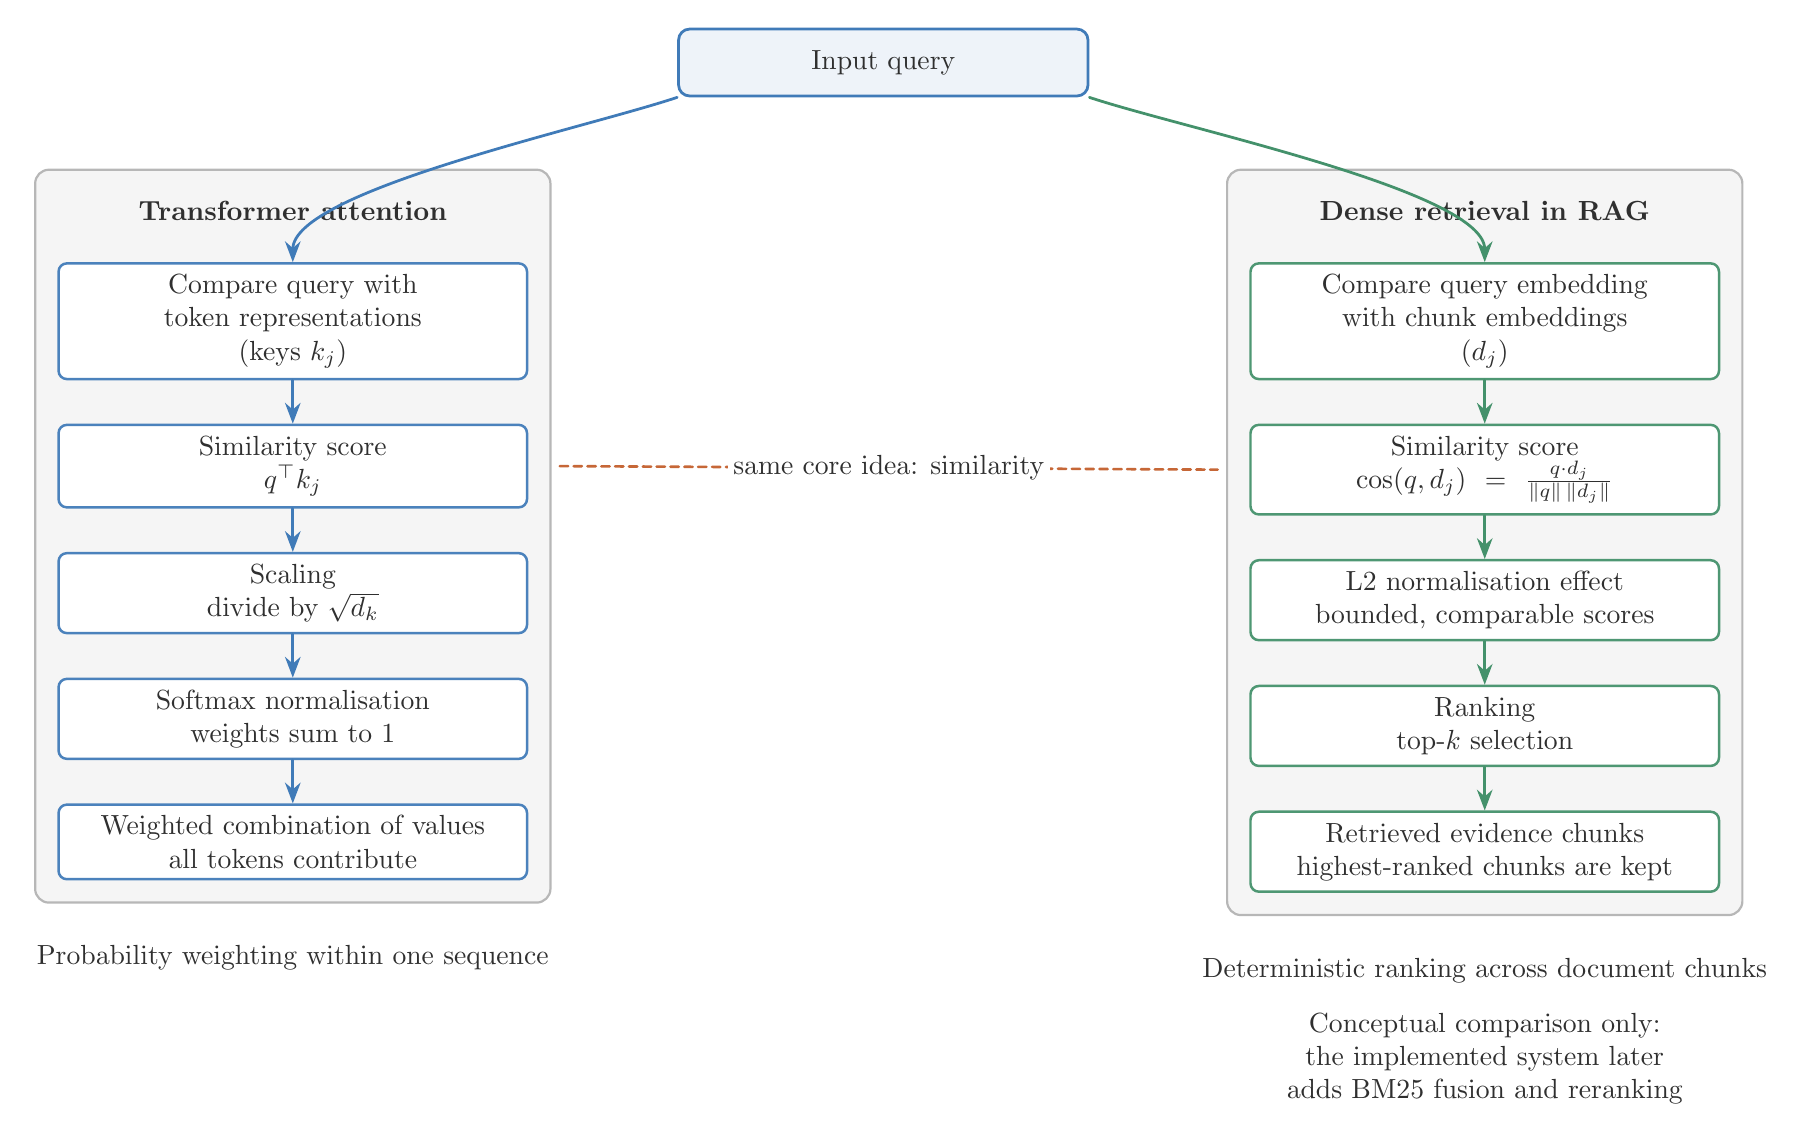
\begin{tikzpicture}[
    >=Stealth,
    font=\rmfamily\normalsize,
    line cap=round,
    line join=round,
    node distance=5.5mm and 16mm,
    panel/.style={draw=framegray, rounded corners=5pt, fill=softgray, inner sep=8pt, line width=0.8pt},
    querybox/.style={draw=attblue!90, fill=attblue!8, rounded corners=4pt, minimum width=5.2cm, minimum height=8.5mm, align=center, line width=1.0pt, text=ink},
    coltitle/.style={font=\rmfamily\bfseries\normalsize, text=ink},
    stepbase/.style={draw=framegray!90, fill=white, rounded corners=3pt, minimum width=5.95cm, minimum height=9.3mm, text width=5.25cm, align=center, inner sep=4pt, line width=0.9pt, text=ink},
    attstep/.style={stepbase, draw=attblue!85},
    ragstep/.style={stepbase, draw=raggreen!85},
    flowblue/.style={->, line width=1.0pt, draw=attblue!90},
    flowgreen/.style={->, line width=1.0pt, draw=raggreen!90},
    foot/.style={font=\rmfamily\normalsize, text=ink, align=center},
    cue/.style={font=\rmfamily\normalsize, text=ink, fill=white, inner sep=2pt}
]

% Query node
\node[querybox] (query) {Input query};

% Titles
\node[coltitle, below left=12mm and 28mm of query] (titleL) {Transformer attention};
\node[coltitle, below right=12mm and 28mm of query] (titleR) {Dense retrieval in RAG};

% Left column
\node[attstep, below=4mm of titleL] (att1) {Compare query with token representations\\(keys $k_j$)};
\node[attstep, below=of att1] (att2) {Similarity score\\$q^{\top}k_j$};
\node[attstep, below=of att2] (att3) {Scaling\\divide by $\sqrt{d_k}$};
\node[attstep, below=of att3] (att4) {Softmax normalisation\\weights sum to 1};
\node[attstep, below=of att4] (att5) {Weighted combination of values\\all tokens contribute};

% Right column
\node[ragstep, below=4mm of titleR] (rag1) {Compare query embedding with chunk embeddings\\($d_j$)};
\node[ragstep, below=of rag1] (rag2) {Similarity score\\$\cos(q,d_j)=\frac{q\cdot d_j}{\|q\|\,\|d_j\|}$};
\node[ragstep, below=of rag2] (rag3) {L2 normalisation effect\\bounded, comparable scores};
\node[ragstep, below=of rag3] (rag4) {Ranking\\top-$k$ selection};
\node[ragstep, below=of rag4] (rag5) {Retrieved evidence chunks\\highest-ranked chunks are kept};

% Panels
\begin{pgfonlayer}{background}
\node[panel, fit=(titleL)(att1)(att2)(att3)(att4)(att5)] (panelL) {};
\node[panel, fit=(titleR)(rag1)(rag2)(rag3)(rag4)(rag5)] (panelR) {};
\end{pgfonlayer}

% Flow arrows from query
\draw[flowblue] (query.south west) .. controls ++(-1.2,-0.4) and ++(0,0.9) .. (att1.north);
\draw[flowgreen] (query.south east) .. controls ++(1.2,-0.4) and ++(0,0.9) .. (rag1.north);

% Downward arrows
\draw[flowblue] (att1) -- (att2);
\draw[flowblue] (att2) -- (att3);
\draw[flowblue] (att3) -- (att4);
\draw[flowblue] (att4) -- (att5);

\draw[flowgreen] (rag1) -- (rag2);
\draw[flowgreen] (rag2) -- (rag3);
\draw[flowgreen] (rag3) -- (rag4);
\draw[flowgreen] (rag4) -- (rag5);

% Similarity cue
\coordinate (cueL) at ($(att2.east)+(4mm,0)$);
\coordinate (cueR) at ($(rag2.west)+(-4mm,0)$);
\draw[densely dashed, line width=0.95pt, draw=accentorange!90] (cueL) -- (cueR);
\node[cue] at ($(cueL)!0.5!(cueR)$) {same core idea: similarity};

% Bottom notes
\node[foot, below=7mm of att5] {Probability weighting within one sequence};
\node[foot, below=7mm of rag5] {Deterministic ranking across document chunks};
\node[foot, below=14mm of rag5, text width=6.1cm] {Conceptual comparison only:\\the implemented system later adds BM25 fusion and reranking};

\end{tikzpicture}
\end{document}
